\newpage
\question
\begin{parts}
\part 
In the Venn diagram, shade the region represented by $P \cap Q^{\prime}$.\\
\begin{center}
        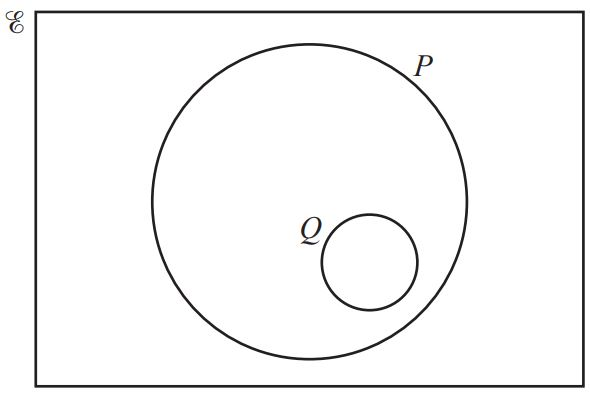
\includegraphics[scale=0.6]{Questions/quiz 18/images/7.JPG}
\end{center}
{\flushright{
\hfill          \makebox[12em]{\dotfill}  [1]}}\\ \\
\part 
A club has 32 members.\\
14 of the members are female and 18 of the members are male.\\
5 of the females have black hair.\\
6 of the males have black hair.\\ \\ 
$E=\{ \text{members of the club} \}$\\
$F=\{$ females $\}$\\
$B=\{$ members with black hair $\}$\\
\begin{center}
        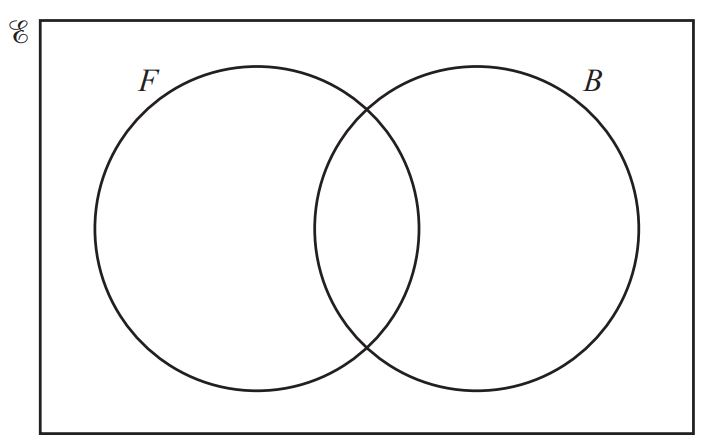
\includegraphics[scale=0.6]{Questions/quiz 18/images/8.JPG}
\end{center} 
Complete the Venn diagram to show this information. \flushright{
          [2]}
\end{parts}